\section{The Hash-and-Resubmit Pattern}

We now introduce a novel design pattern for Solidity smart contracts that
results into significant gas optimization due to the elimination of expensive
storage operations. We first introduce our pattern, and illustrate how smart
contracts benefit from using it. Then, we proceed to integrate our pattern
in the NIPoPoW protocol, and we analyze the performance in comparison with
previous work~\cite{gglou}.

\noindent
\textbf{Motivation.}
It is essential for smart contracts to store data in the blockchain. However,
interacting with the storage of a contract is among the most expensive
operations of the EVM~\cite{wood, buterin}. Therefore, only necessary data
should be stored and redundancy should be avoided when possible. This is
contrary to conventional software architecture, where storage is considered
cheap. Usually, data access performance in traditional systems is
measured with respect to time and space. In Ethereum, however, performance is related to gas
consumption. Access to persistent data costs a substantial amount of gas, which
has a direct correspondence to a monetary cost.
% One way to mitigate gas cost of reading variables
% from the blockchain is to declare them as public. This leads to the creation of a
% \emph{getter} function in the background, allowing free access to the value of
% the variable. But this treatment does not prevent the initial population of
% storage data and write operations which are significantly expensive for large
% sizes of data.

% By using the \emph{hash-and-resubmit} pattern, large structures are omitted
% from storage entirely, and are contained in memory. When a function call is
% performed, the signature and arguments of the function are included in the
% transactions field of the body of a block. The contents of blocks are public to
% the network, therefore this information is locally available to full nodes. By
% simply observing blocks, a node retrieves data sent to the contract by other
% users. To interact publicly with this data without the utilization storage, the
% node \emph{resends} the observed data to the blockchain. The concept of
% resending data is redundant in conventional systems. However, this technique
% is very efficient to use in Solidity due to the significantly lower gas cost
% of memory operations in relation with storage operations.

\noindent \textbf{Related patterns.} Towards implementing gas-efficient smart
contracts~\cite{contract-opt-1, contract-opt-2, slither, madmax}, several
methodologies have been proposed. In order to eliminate storage operations
using data signatures, the utilization of IPFS~\cite{ipfs} has been
proposed~\cite{ipfs-1,ipfs-2}. However, these solutions do not address
\emph{availability}, which is one of our main requirements. Another solution
uses logs~\cite{logs} to replace storage in a similar manner, sparing a great
amount of gas. However, this approach does not address consistency, which is
also one of our critical targets. Lastly, there have been proposals~\cite{memory-array}
to replace storage read operations, but they do not address write operations.


\begin{figure*}[h]
    \begin{center} 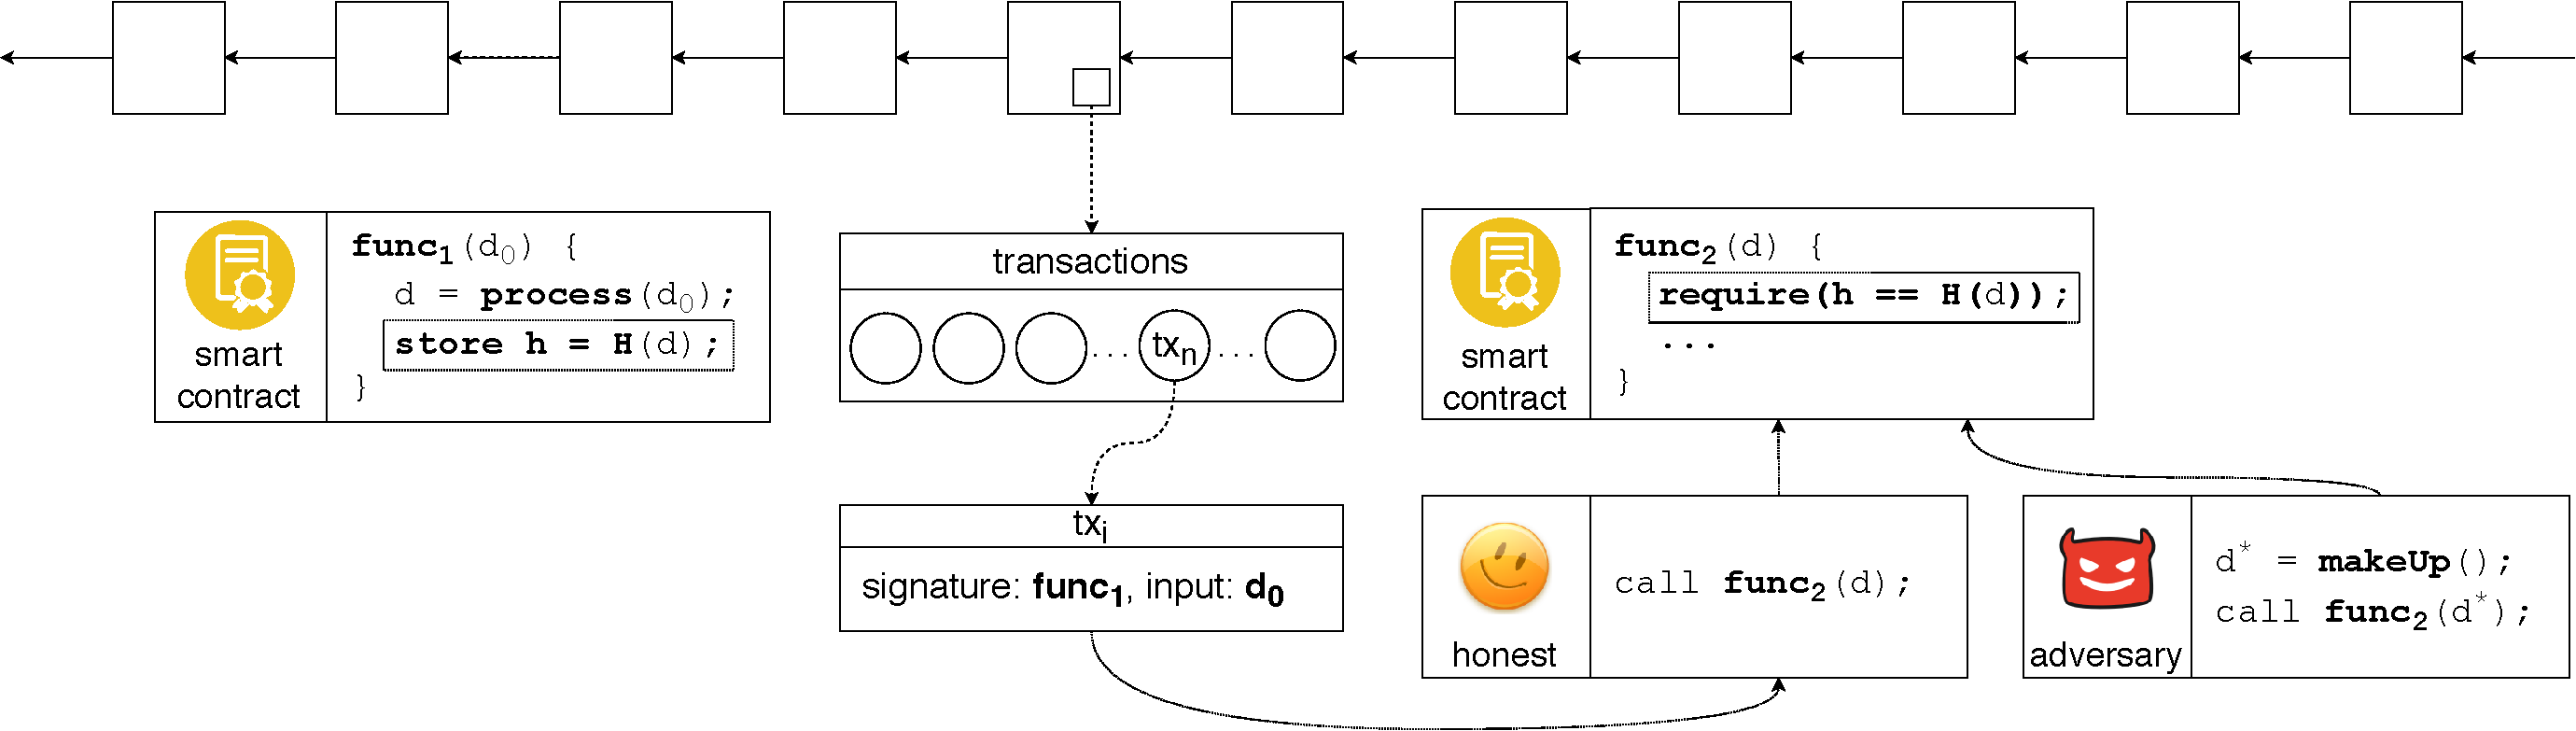
\includegraphics[width=0.8\textwidth]{figures/har-pattern.pdf}
    \end{center}

    \caption{The \emph{hash-and-resubmit} pattern. First, an invoker calls
        \proc$_1$($\data_0$). Then $\data_0$ is processed \emph{on-chain} and
        $\data$ is generated. The commitment to $\data$ is stored in the
        blockchain as the digest of a hash function $H(\cdot)$. Then,
        a full node that observes invocations of $\proc_1$ retrieves $\data_0$,
        and generates $\data$ by performing the respective processing on
        $\data_0$ \emph{off-chain}. An adversarial observer dispatches
        $\datas$, where $\datas$$\neq$$\data$. Finally, the nodes invoke
        $\proc_2$(.). In $\proc_2$, the validation of input data is performed,
        reverting the function call if the hash of the input does not
        match with the stored commitment. By applying
        a \emph{hash-and-resubmit pattern}, only the fixed-size commitment of
        $\data$ is stored to the contract's state, replacing arbitrarily large
        structures.}

        \label{fig:har-pattern}
\end{figure*}

\noindent
\textbf{Applicability.}
To benefit from the \emph{hash-and-resubmit} pattern, an application needs to
meet the following requirements:

\begin{enumerate}
    \item The application is a Solidity smart contract.
    \item Read/write operations are performed in large arrays that exist in
        storage. Using the pattern for variables of small size may result in
        negligible gain or even performance loss.
    \item A full node observes function calls to the smart contract.
\end{enumerate}

\noindent \textbf{Participants and collaborators.} The first participant is the
smart contract $\contract$ that accepts function calls. Another participant is
the invoker $\invoker$, who dispatches a large array $\data_0$ to $\contract$
via a function \texttt{\proc$_1$}($\data_0$). Upon submission, $\data_0$ is
potentially processed in $\proc_1$, resulting to $\data$. The last participant
is the observer $\observer$, who is a full node that observes transactions
towards $\contract$ in the blockchain. This is possible because nodes maintain
the blockchain locally. After observation, $\observer$ retrieves data $\data$.
Since this is an off-chain operation, a malicious $\observer$ potentially
alters $\data$ before interacting with $\contract$. We denote the
potentially modified $\data$ as $\datas$. Finally, $\observer$ acts as an
invoker by making a new call to $\contract$, \texttt{\proc$_2$}($\datas$). The
verification that $\data = \datas$, which is a prerequisite for the secure
functionality of the underlying contract, forms a part of the pattern and is
performed in \texttt{\proc$_2$}.

\noindent \textbf{Implementation.} The implementation of this pattern is
divided in two parts. The first part covers how $\datas$ is retrieved by
$\observer$, whereas in the second part the verification of $\data=\datas$ is
realized. The challenge here is twofold:

\begin{enumerate}

    \item Availability: $\observer$ must be able to retrieve $\data$ without
        the need of accessing on-chain data.

    \item Consistency: $\observer$ must be prevented from dispatching $\datas$
        that differs from $\data$ which is a product of the originally submitted
        $\data_0$.

\end{enumerate}

\noindent
The \emph{hash-and-resubmit} technique is performed in two
stages to face these challenges: (a) the \emph{hash} phase, which addresses
\emph{consistency}, and (b) the \emph{resubmit} phase which addresses
\emph{availability} and \emph{consistency}.

\noindent \textsf{Addressing availability:} During the \emph{hash} phase,
$\invoker$ makes the function call \texttt{\proc}$_1$($\data_0$). This
transaction, which includes a function signature (\texttt{\proc$_1$}) and the
corresponding data ($\data_0$), is confirmed in a block by a miner. Due to
blockchain's transparency, the observer $\observer$ of \texttt{\proc}$_1$
retrieves a copy of $\data_0$ from the calldata, without the need of accessing contract data. In
turn, $\observer$ performs \emph{locally} the same set of on-chain instructions
operated on $\data_0$, generating $\data$. Thus, availability is addressed
through observability.

\noindent \textsf{Addressing consistency:} We prevent an adversary $\observer$
from dispatching data $\datas\neq\data$ by storing the \emph{commitment} of
$\data$ in the contract's state during the execution of \texttt{\proc$_1$(.)} by
$\invoker$. In the context of Solidity, a commitment is the
digest of the structure's \emph{hash}. The pre-compiled \texttt{sha256} is
convenient to use in Solidity; however we can make use of any cryptographic
hash function $H(\cdot)$: \[\textsf{hash} \gets \textsf{H}(\textsf{d})\]
Then, in \emph{rehash} phase, the verification is performed by comparing the
stored digest of $\data$ with the digest of $\datas$:
\[\textsf{require}(\textsf{hash} = \texttt{H}(\datas))\] \noindent In Solidity,
the size of this digest is 32 bytes. To persist such a small value in the
contract's memory only adds a small constant gas overhead. We illustrate
the application of the \emph{hash-and-resubmit} pattern in
Figure~\ref{fig:har-pattern}.

\noindent \textbf{Sample.} We now demonstrate the usage of the
hash-and-resubmit pattern with a simplistic example. We create a smart contract
that orchestrates a game between two players, $\pla$ and $\plb$. The winner is
the player with the most valuable array. The interaction between players
through the smart contract is realized in two phases: (a) the submit phase and
(b) the contest phase.

\noindent \textsf{Submit phase:} $\pla$ submits an N-sized array, $\arra$, and
becomes the $\holder$ of the contract.

\noindent \textsf{Contest phase:} $\plb$ submits $\arrb$. If the result of
\textsf{compare}($\arrb$, $\arra$) is \true, then $\plb$ becomes the holder. We
provide a simple implementation for \textsf{compare}, but we can consider any
notion of comparison, since the pattern is abstracted from such implementation
details.

We make use of the \emph{hash-and-resubmit} pattern by prompting $\plb$ to
provide \emph{two} arrays to the contract during contest phase: (a) $\arras$,
which is the originally submitted array by $\pla$, possibly modified by $\plb$,
and (b) $\arrb$, which is the contesting array.

We provide two implementations of the above described game.
In Algorithm~\ref{alg:game-storage} we display the storage implementation,
while in Algorithm~\ref{alg:game-memory} we show the implementation
leveraging the \emph{hash-and-resubmit} pattern.

\begin{algorithm}
    \caption{\label{alg:game-storage}\textsf{best array} using storage}
    \begin{algorithmic}[1]

    \Contract{best-array}
        \State{$\textsf{best} \gets \emptyset$;
               $\textsf{holder} \gets \emptyset$}
        \Function{\sf submit}{$a$}
        \State \textsf{best} $\gets a$
            \Comment{array saved in storage}
            \State \textsf{holder $\gets$ msg.sender}
        \EndFunction

        \Function{\sf contest}{$a$}
            \State \textsf{require}(\textsf{compare}($a$))
            \State \textsf{holder} $\gets$ \textsf{msg.sender}
        \EndFunction

        \Function{\sf compare}{$a$}
            \State \textsf{require}($|a|$ $\geq$ $|$\textsf{best}$|$)
            \For{$i$ \textbf{in} $|$\textsf{best}$|$}
            \State \textsf{require}($a[i]$ $\geq$ \textsf{best}[i])
            \EndFor
            \State \Return{true}
        \EndFunction
        \EndContract
        \vskip8pt
    \end{algorithmic}
\end{algorithm}

\begin{algorithm}
    \caption{\label{alg:game-memory}\textsf{best array} using hash-and-resubmit pattern}
    \begin{algorithmic}[1]
        \Contract{best-array}
        \State{$\textsf{hash} \gets \emptyset$;
               $\textsf{holder} \gets \emptyset$}

        \Function{\sf submit}{$\arra$}
        \State $\textsf{hash} \gets \textsf{H}(\arra)$
            \Comment{hash saved in storage}
            \State \textsf{holder} $\gets$ \textsf{msg.sender}
        \EndFunction

    \Function{\sf contest}{$\arra^*$, $\arrb$}
    \State \textsf{require}(\textsf{hash256}($\arra^*$) $=$ $hash$)
        \Comment{validate $\arra^*$}
        \State \textsf{require}(\textsf{compare}($\arra^*$, $\arrb$))
        \State \textsf{holder} $\gets$ \textsf{msg.sender}
    \EndFunction
    \Function{\sf compare}{$\arra^*$, $\arrb$}
        \State \textsf{require}($|\arra^*|$ $\geq$ $|\arrb|$)
        \For{$i$ \textbf{in} $|\arra^*|$}
            \State \textsf{require}($\arra^*[i] \geq \arrb[i]$)
        \EndFor
    \EndFunction
    \State \Return{true}
    \EndContract
    \vskip8pt
    \end{algorithmic}
\end{algorithm}


\noindent \textbf{Gas analysis.} The gas consumption of the two above
implementations is displayed in Figure~\ref{fig:har-example}. By using the
\emph{hash-and-resubmit} pattern, the aggregated gas consumption for
\textsf{submit} and \textsf{contest} is decreased by 95\%. This significantly
affects the efficiency and applicability of the contract. Note that the storage
implementation exceeds the Ethereum block gas limit ($10{,}000{,}000$ gas as of
June 2020), for arrays of size 500 and above, contrary to the optimized
version, which consumes approximately only $1/10^{th}$ of the block gas limit
for arrays of $1{,}000$ elements.

\begin{figure}[!h]
\vspace*{-5mm}
\begin{center}
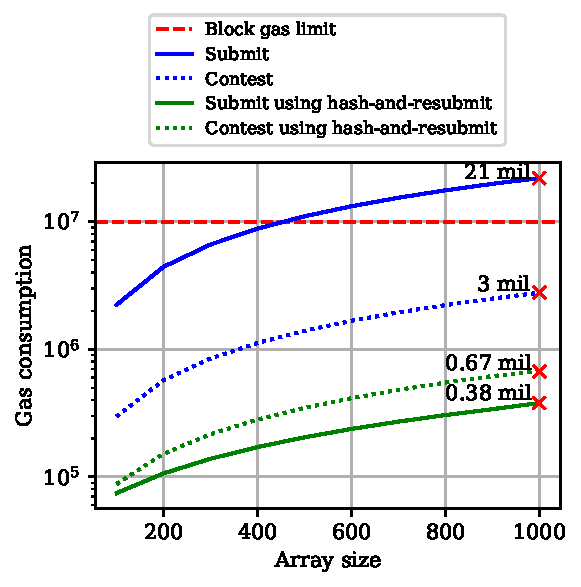
\includegraphics[width=0.9 \columnwidth]{figures/har-example.pdf}
\end{center}
\vspace*{-5mm}
\caption{Gas-cost reduction of Algorithm~\ref{alg:game-storage} using the \emph{hash-and-resubmit} pattern (lower
is better). By avoiding gas-heavy storage operations, the aggregated cost of
\textsf{submit} and \textsf{contest} is decreased by 95\%.}
\label{fig:har-example}
\vspace*{-5mm}
\end{figure}

\noindent \textbf{Consequences.} The consequence of applying the
\emph{hash-and-resubmit} pattern is the circumvention of storage,
a benefit that saves a substantial amount of gas, especially when
stored structures are large. Therefore, smart contracts that exceed the
Ethereum block gas limit and benefit sufficiently from the alleviation of
storage can become practical.

\noindent \textbf{Known uses.} To our knowledge, we are the first to address
consistency and availability by combining blockchain's transparency with commitments
in a manner that eliminates storage from smart contracts.

\noindent \textbf{Enabling NIPoPoWs.} We now present how the
\emph{hash-and-resubmit} pattern is used in the context of the NIPoPoW
superlight client. The NIPoPoW verifier adheres to a submit-and-contest schema
where the inputs of the functions are arrays that are processed on-chain, and a
node observes function calls towards the smart contract.  Therefore, it
makes a suitable case for our pattern.

In the \emph{submit} phase, a \emph{proof} is submitted. In the case the proof is fraudulent, it
is contested by another user in the \emph{contest} phase. The contester is a node
that monitors the traffic of the verifier contract. The input of the \textsf{submit}
function includes the submit proof ($\pis$) that claims the occurrence of an
\emph{event} ($e$) in the source chain, and the input of the \textsf{contest}
function includes a contesting proof ($\pic$). A successful contest of $\pis$
is realized when $\pic$ has a better score~\cite{nipopows}. In this section, we
will not examine the score evaluation process since it is irrelevant to the
pattern. The size of proofs is dictated by the value $m$. We adopt the recommended~\cite{nipopows}
parameter value $m = 15$.

In previous work, NIPoPoW proofs are maintained on-chain, resulting in
extensive storage operations. In our implementation, proofs are not stored on-chain, and $\pis$
is retrieved by the contester from the calldata. Since we
assume a trustless network, $\pis$ can be altered by an adversarial contester. We denote
the potentially changed $\pis$ as $\pisa$. In the \emph{contest} phase, $\pisa$ and
$\pic$ are dispatched in order to enable the \emph{hash-and-resubmit} pattern.

For our analysis, we create a blockchain similar to the Bitcoin chain with the
addition of the interlink structure in each block~\cite{gglou}. Our experimental chain
spans 650,000 blocks, representing a slightly larger chain than
Bitcoin\footnote{Bitcoin spans $633{,}022$ blocks as of June 2020. Metrics by
https://www.blockchain.com/}. From the tip of our chain, we branch two
sub-chains that span 100 and 200 additional blocks respectively, as illustrated
in Figure~\ref{fig:chains}. Then, we use the smaller chain to create $\pis$,
and the larger chain to create $\pic$. We apply the protocol by submitting
$\pis$, and contesting with $\pic$. The contest is successful, since $\pic$
represents a chain consisting of a greater number of blocks than $\pis$.
We select this setting as it
provides maximum code coverage, and it describes the most gas-heavy scenario
for the verifier.

In Algorithm~\ref{alg:har-nipopow} we show how the \emph{hash-and-resubmit} pattern
is leveraged by our modified NIPoPoW client.

\begin{figure}[!h]
    \begin{center}
        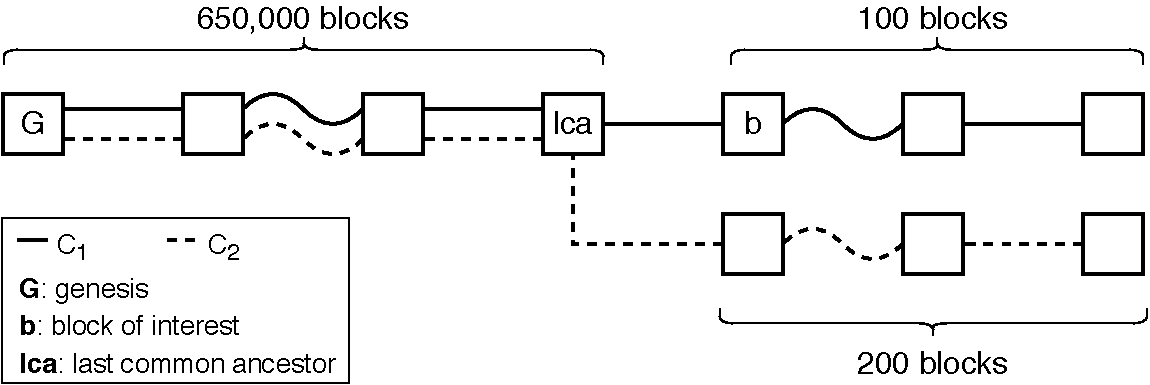
\includegraphics[width=1\columnwidth]{figures/nipopow-subm-cont}
    \end{center}
    \caption{Forked chains for our gas analysis.}
    \label{fig:chains}
\vspace*{-3mm}
\end{figure}

In Figure~\ref{fig:har-nipopow}, we illustrate how \emph{hash-and-resubmit}
improves client performance compared to previous work. The graph
illustrates the aggregated cost of the \emph{submit} and \emph{contest} phases for
each implementation. We observe that, by using the \emph{hash-and-resubmit}
pattern, we improve the gas consumption of the contract by 50\%. This
is a decisive step towards creating a practical superlight client.

Note that, in our graph, gas consumption generally follows an ascending trend; however it
is not monotonically increasing. This is due to the fact that
NIPoPoWs are probabilistic structures, the size of which is determined by the
distribution of superblocks within the underlying chain. A proof that is
constructed for a chain of a certain size can be larger than a proof
constructed for a slightly smaller chain, sometimes resulting in a slight decrease
of gas consumption between consecutive values of proof sizes.

\newcommand{\genesis}{\textsf{G}}

\begin{algorithm}
    \label{alg:har-nipopow}
    \caption{The \textsf{NIPoPoW} client using hash-and-resubmit pattern}
    \begin{algorithmic}[1]

    \Contract{crosschain}
    \State $\textsf{events} \gets \bot;$ $\genesis \gets \bot$
    \Function{\sf initialize}{$\genesis_{remote}$}
        \State \genesis $\gets \genesis_{remote}$
    \EndFunction
    \Function{\sf submit}{$\pis$, $e$}
        \State \textsf{require}($\pis$[0] = $\genesis$)
        \State \textsf{require}($\textsf{events$[e]$} = \bot$)
        \State \textsf{require}($\textsf{valid-interlink}(\pi)$)
        \State \textsf{DAG} $\gets$ \textsf{DAG} $\cup$ $\pis$
        \State \textsf{events$[e]$.hash} $\gets$ \textsf{H}($\pis$)
        \Comment{enable pattern}
        \State \textsf{ancestors} $\gets$ \textsf{find-ancestors()}
        \State \textsf{events$[e]$.pred} $\gets$
            \textsf{evaluate-predicate}(\textsf{ancestors}, e)
        \State \textsf{ancestors} $=$ $\bot$
    \EndFunction
    \Function{\sf contest}{$\pisa$, $\pic$, $e$}
        \Comment{provide proofs}
        \State \textsf{require}(\textsf{events$[e]$.hash} $=$ \textsf{H}($\pisa$))
        \Comment{verify $\pisa$}
        \State \textsf{require}($\pic$[0] = $\genesis$)
        \State \textsf{require}(\textsf{events}$[e]$ $\ne$ $\bot$)
        \State \textsf{require}(\textsf{valid-interlink}($\pi_{cont}$))
        \State $lca$ = \textsf{find-lca}($\pisa$, $\pic$)
        \State \textsf{require}(\textsf{score}($\pic[:lca]$)
            $>$ \textsf{score}($\pisa[:lca]$))
        \State \textsf{DAG} $\gets$ \textsf{DAG} $\cup$ $\pic$
        \State \textsf{ancestors} $\gets$ \textsf{find-ancestors}(\textsf{DAG})
        \State \textsf{events$[e]$.pred} $\gets$
            \textsf{evaluate-predicate}(\textsf{ancestors}, $e$)
        \State \textsf{ancestors} $=$ $\bot$
    \EndFunction
    \EndContract
    \vskip8pt
    \end{algorithmic}
\end{algorithm}



\begin{figure}[!h]
    \begin{center}
        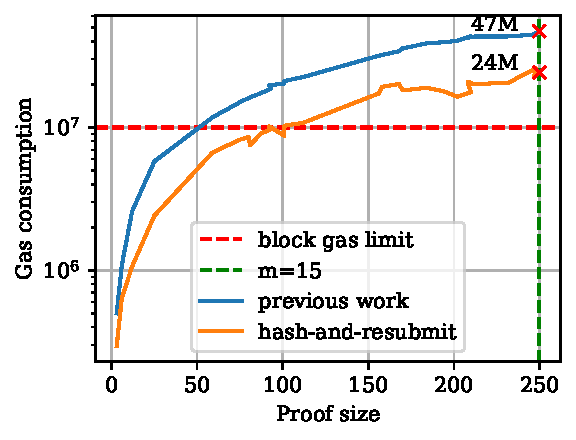
\includegraphics[width=0.9\columnwidth]{figures/har-nipopows.pdf}
    \end{center}
\vspace*{-5mm}
    \caption{Gas consumption of our NIPoPoWs verifier enhanced with hash-and-resubmit
        compared to previous work (lower is better) using a secure value of $m$.
        Gas consumption is decreased by approximately 50\%.}
    \label{fig:har-nipopow}
\vspace*{-5mm}
\end{figure}
